% manually add a new line so the ToC for this chapter starts on a new page
\addtocontents{toc}{\newpage}
\chapter{Evaluation of the Prototype}
\label{chap:evaluation-of-the-prototype}
In this chapter I present the measurements of various system functions and the runtime characteristics of the prototype framework.

Due to the underlying approached, the presented framework has its limitations and trade-offs. Processing one file at a time makes the approach incremental with file-level granularity, potentially saving time on the whole, but takes a large amount of time integrating the parser into the system. The approach also requires less memory during the parsing phase, but takes more time once every file was processed and the connecting phase takes place.

\section{Benchmarking Environment}
In order to make sure that the measurements are reproducible, and are not affected by user input or other environmental events, the measurements were performed in the cloud. In this section I detail the hardware and software configurations for the benchmarks.

\subsection{Virtual Machine Configuration}
The benchmarks were carried out in a Microsoft Azure virtual machine~\cite{azure-vm}. Since the approach utilizes a persisted graph database with in-memory caching, I have chosen a configuration with moderate amount of memory for a server and high IO performance.

The D-series virtual machines were designed with data-intensive use-cases in mind, like Big Data and Analytics.~\cite{d-series} The virtual machine instance was located in the West Europe region.

The \emph{Standard DS3\_v2} configuration consists of the following:
\begin{itemize}[topsep=0pt]
  \item 4 CPU cores (Intel(R) Xeon(R) CPU E5-2673 v3 @ 2.40GHz --- \emph{reported})
  \item 14 GB memory
  \item 8 data disks
  \item 12800 maximum IOPS
  \item 28 GB local SSD
\end{itemize}

\subsection{Software Configuration}
The results of the benchmarks can also be affected by the software configuration. I have selected the preconfigured \emph{Ubuntu Server} virtual machine with the following properties and modifications:

\begin{itemize}[topsep=0pt]
  \item Ubuntu 16.04.1 LTS (GNU/Linux 4.4.0-42-generic x86\_64)
  \item Oracle Java(TM) SE Runtime Environment (build 1.8.0\_111-b14)
  \item Java Virtual Machine with 2 GB minimum and 12 GB maximum heap space
  \item bash benchmarking script with curl
\end{itemize}

\subsection{Framework Dependencies}
The prototype of the framework was based on changing and rapidly developed dependencies. Both Neo4j and Shift had version and API changes, so I chose to freeze the versions at a working state and use them for the measurements.

Neo4j was freezed at the first released 3.0 version: 3.0.0. At the time of writing this report it is at version 3.0.6, with 3.1 being available as a beta. Shift was freezed at 2.2.0 with custom modifications.

I needed to perform some modifications on the Shift source code, which were later merged\footnote{\small\url{https://github.com/shapesecurity/shift-java/pull/101}} to the Shift repository.


\section{Benchmark Cases}
In this section I iterate over the various benchmark cases, present them in detail, introduce the results of the measurements and evaluate the results.

\subsection{Graph Database Initialization}
The framework uses the Neo4j server in embedded mode (instead of a standalone configuration). This means that the server is started with the framework and at the first usage it needs initialization.

While the following benchmarks are prepared with initialized databases, I have measured the time required to prepare an empty database. This is measured by deleting the database folder, restarting the application and executing a simple query counting the nodes.

The database requires on average 996, median 1015 milliseconds to initialize\footnote{936, 945, 1010, 1019, 1022, and 1042 milliseconds in the 6 runs, respectively}.

\subsection{Source to Graph Transformation}
After the database has been initialized, it can receive content. This transformation process is one of the most time-consuming workflows. Here the source code of the file is read from the disk or the memory, transferred to the server. It is then parsed using the Shift parser, extended with the scope analyzer and stored in the database while iterating over every node.

\begin{figure}[!htb]
  \centering
  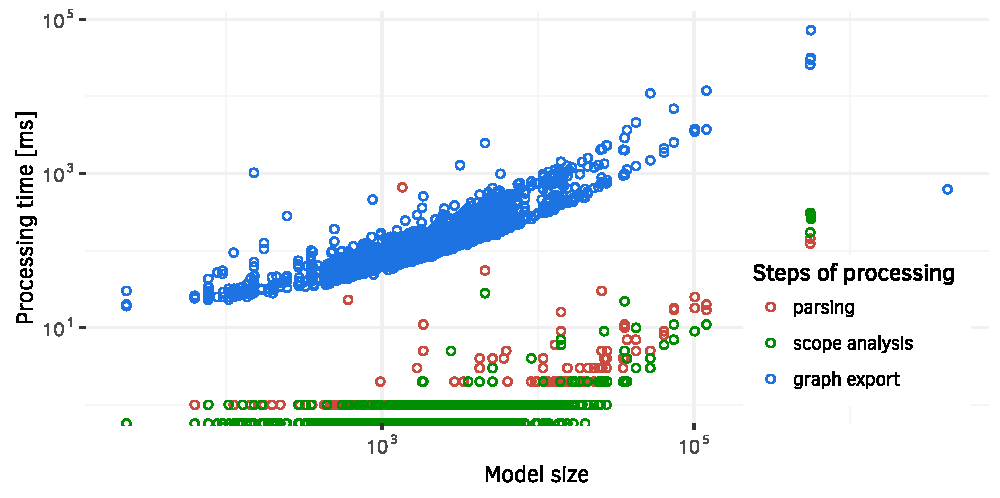
\includegraphics[width=\textwidth]{import-steps.pdf}
  \caption{The characteristics of the import steps.}
  \label{fig:import-steps}
\end{figure}

\Cref{fig:import-steps} shows the characteristics of these three steps. Since even the longest source codes can be written in one line, instead of the source lines of code I have chosen the number of nodes in the transformed subgraph (model size) as the horizontal axis. The vertical axis represents the time (in milliseconds) required to perform the given transformation step. Note that both axes are logarithmic.

In order to present an accurate and wide-range measurement, I have selected the repository of the Tresorit web client~\cite{tresorit-webclient}. The current version of this repository contains 780 JavaScript files, with 75\,907 lines of actual code in total. This results in 8\,437\,838 graph nodes.

Since the source code contains language elements not yet standardized, I translated the source code to conform ES5 before it is parsed by the Shift parser. This step is not calculated in the benchmark. The resulting files are then imported into the database one-by-one, sequentially, thus the parallel optimizations are not present in this measurement.

Based on~\Cref{fig:import-steps} the time requirement of the parsing and scope analysis steps are negligible compared to the third step. Iterating and storing the elements of the ASG in the graph database shows polynomial correlation with the size of the graph. It is also visible that most of the files are parsed under one second, which indicates that it can be employed in continuous and everyday development.

These results are based on two separate, sequential, full import of the source code repository, containing 780 files.

%\subsection{Connecting the Subgraphs}
% TODO write or hide

\subsection{Dead Code Search}
Searching for dead code snippets consists of two phases: first, the call graph has to be prepared, then the graph is queried for unreachable code. Since the transformation rules and queries are far from complete and are not covering every code model scenario, this measurement can only report the characteristics of the current implementation.

\begin{figure}[!htb]
  \centering
  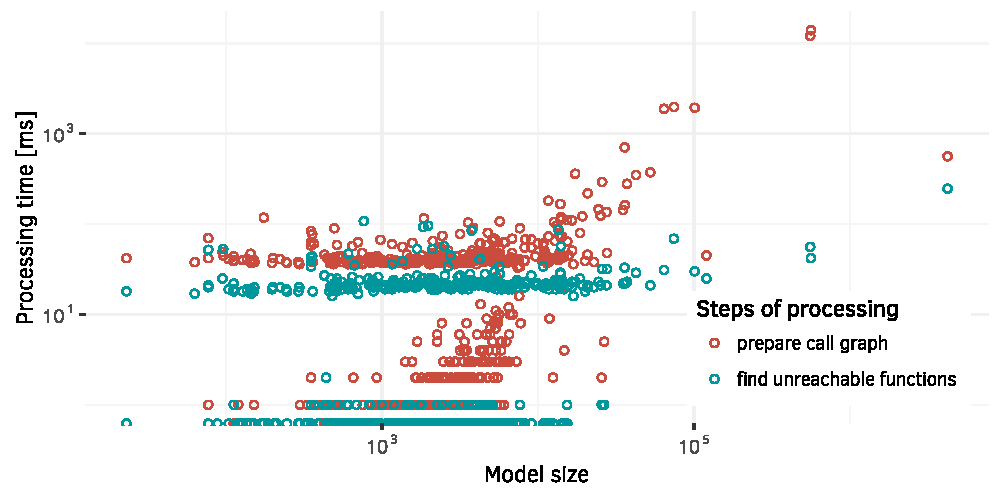
\includegraphics[width=\textwidth]{deadcode-search.pdf}
  \caption{The characteristics of dead code search.}
  \label{fig:deadcode-search}
\end{figure}

\Cref{fig:deadcode-search} shows at least two horizontal clusters for both steps. On the bottom, there are files that probably contain none or only a few nodes processed by the queries. Based on the figure and manual testing, the characteristics of the upper cluster is to be expected when the transformation rules provide full coverage, resulting in constant runtime for most cases.

The results are based on one-time, file-by-file import and dead code search of the source code repository, containing 780 files.

\subsection{ASG to CFG Transformation}
In order to measure the characteristics of the CFG transformation, I have imported the source files of the Tresorit web client one-by-one and executed the CFG transformation queries at a time.

\begin{figure}[!htb]
  \centering
  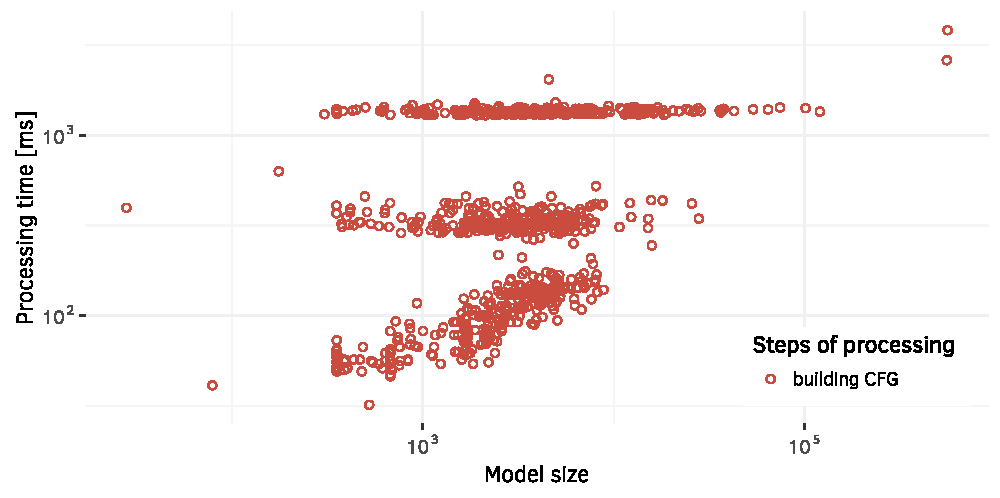
\includegraphics[width=\textwidth]{build-cfg.pdf}
  \caption{The characteristics of building the CFG.}
  \label{fig:build-cfg}
\end{figure}

\Cref{fig:build-cfg} shows that the measurements are clustered into three parts. There are at least two explanations for this:

\begin{itemize}[topsep=0pt]
  \item The number of CFG transformations implemented in the prototype framework is low. Since there are measurements in every cluster for a great amount of model sizes, it is possible that the composition of the files are different in each cluster.

  This would mean that the top cluster --- implementing business logic --- contains more nodes to transform, while the files in the bottom cluster --- mostly describing interfaces and proxies --- contain less.

  \item The transformation is executed in a parallel manner. If two transformations cause a deadlock in the database, they are canceled and tried again later. It is also possible that subgraphs containing more transformable nodes by the framework are processed slower. The slower the transformations are, the more deadlocks may happen, resulting in slower overall performance.
\end{itemize}

It is also unexpected to have the top two clusters show no correlation with the size of the resulting graph size. This phenomenon can be explained with the reasons above or with the way Neo4j executes declarative transformations.

The results are based on one-time, file-by-file import and transformation of the source code repository, containing 780 files. Since the CFG transformation in the framework is far from finished, deeper examination of the results is subject to future work.

\subsection{Incremental Processing}
Since the framework processes the changes file-by-file, it is possible to execute the analysis in an incremental fashion with file-level granularity. After every file has been processed and a new changeset is present, it is only required to update and process the modified file and the affected graph parts.

\begin{figure}[!htb]
  \centering
  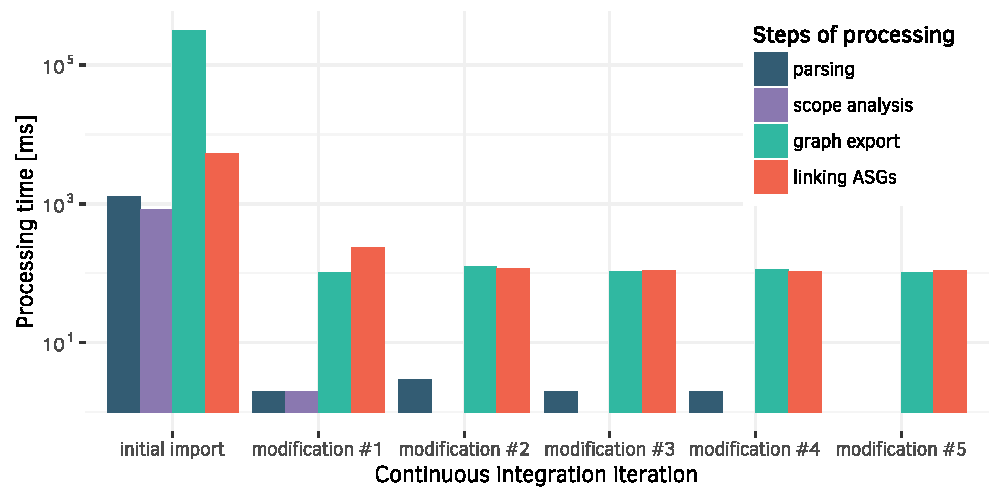
\includegraphics[width=\textwidth]{CI-iteration-benchmark.pdf}
  \caption{Runtime measurements of the execution of the analysis for sequential modifications.}
  \label{fig:CI-iteration-benchmark}
\end{figure}

\Cref{fig:CI-iteration-benchmark} details the execution times for each step during the initial and the subsequent change propagations. These all consist of the same steps: 1)~the source code is parsed, then 2)~scope analysis is applied, and 3)~the resulting ASG is stored in the graph database, finally 4)~the inserted subgraph is linked to the already stored nodes, imitating the JavaScipt module import-export resolution.

The initial import was executed first. After all 780 files have been processed one-by-one, the import-export linking was executed once. Subsequent modifications was simulated by removing and reprocessing a file with one of the most \code{import} statements (thus resulting in more work for the linking transformation). After each \emph{modification} the linking transformation was applied.

It is visible that the incremental approach for the complete process is faster by three orders of magnitude. The linking step itself is faster by one order of magnitude for linking only one file to the others. (Please note that along with the previous figures, \Cref{fig:CI-iteration-benchmark} is logarithmically scaled on the vertical axis.)


\section{IDE Integration}
\label{sect:ide-integration}
Besides executing measurements, I also created a plugin for Visual Studio Code (introduced in~\Cref{sect:visual-studio-code}) that sends the content of the open file to the framework, when the file is modified and saved. Then it requests the results of the dead code search, and conviniently displays it using the API provided by Visual Studio Code.

\begin{figure}[!htb]
  \centering
  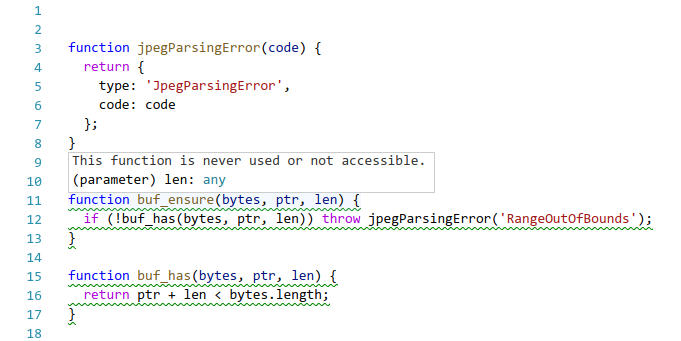
\includegraphics[width=\textwidth]{vsc-integration}
  \caption{Proof-of-concept plugin integration in an industrial case study.}
  \label{fig:vsc-integration}
\end{figure}

\Cref{fig:vsc-integration} shows the proof-of-concept plugin integration displaying dead code warnings for a file in an industrial case study. The previously introduced results in~\Cref{fig:dead-code-result} show that the approach was able to find circular references without incoming calls and report the clique, without user input. To validate the results, I have manually checked the presented warnings.


\section{Threats to Validity}
\label{sect:evaluation-threats}
Although I carefully designed and executed each measurement, there might have been factors beyond control that influence the results yielded. In this section, I try to list the possible mistakes and also discuss the steps taken to mitigate their effects.

\subsection{Benchmarking in the Cloud} As a multiple access system, the virtual servers in the cloud can be easily affected by neighboring virtual machines using the same resources. The virtual machine manager can also limit the usage of these resources, if the machines disturb other ones. One can neither control the resources assigned to the machines, nor influence their precise geolocation and connections.

My mitigation strategy is to run the benchmarks multiple times and treat their median as the representative value, or import a larger codebase with file sizes varying from a few to hundreds of lines.

\subsection{Methodological Mistakes} It is possible that I made mistakes while implementing the approach. It may not adhere to the specification correctly, perform the transformations correctly or measure correctly.

To check the validity of the results, I checked the results manually and with others tools.
